%\documentclass[tikz, border=10pt]{standalone}
\tikzset{
    vertex/.style = {
        circle,
        fill            = black,
        outer sep = 2pt,
        inner sep = 1pt,
    }
}

%\begin{document}

\newcommand{\myfun}[2] {$fun^{#1}_{#2}$}
  
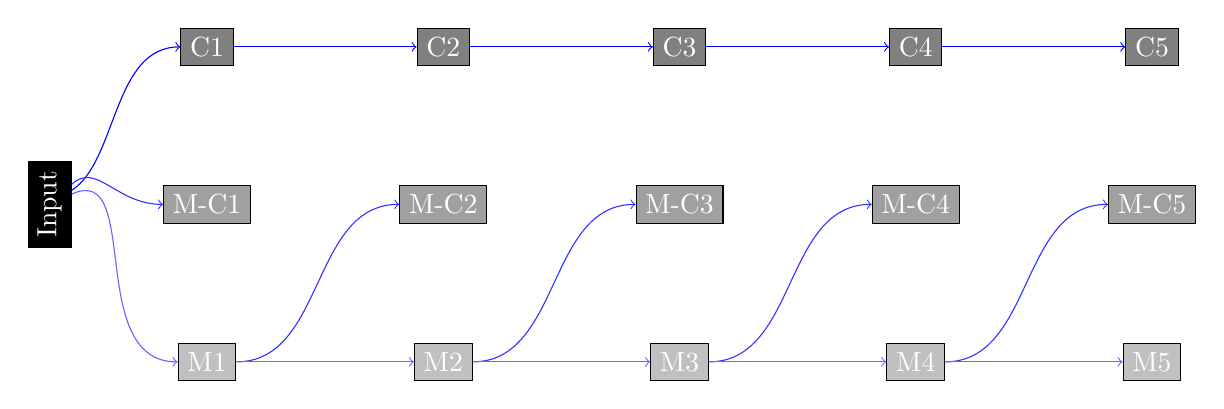
\begin{tikzpicture}
  % Cases
  \definecolor{lgray}{RGB}{192,192,192}
  \definecolor{ngray}{RGB}{160,160,160}
  \definecolor{dgray}{RGB}{128,128,128}
  % Cases
  \definecolor{lblue}{RGB}{102,102,255}
  \definecolor{nblue}{RGB}{51,51,255}
  \definecolor{dblue}{RGB}{0,0,255}
% Input node
\node[draw,fill=black,text=white,rotate=90] (Input) at (2,2) {Input};  
  
% Matlab nodes
\node[draw,fill=lgray,text=white] (funM1) at ( 4,0) {\myfun{M}{1}};
\node[draw,fill=lgray,text=white] (funM2) at ( 7,0) {\myfun{M}{2}};
\node[draw,fill=lgray,text=white] (funM3) at (10,0) {\myfun{M}{3}};
\node[draw,fill=lgray,text=white] (funM4) at (13,0) {\myfun{M}{4}};
\node[draw,fill=lgray,text=white] (funM5) at (16,0) {\myfun{M}{5}};

% MC nodes
\node[draw,fill=ngray,text=white] (funMC1) at ( 4,2) {\myfun{M-C}{1}};
\node[draw,fill=ngray,text=white] (funMC2) at ( 7,2) {\myfun{M-C}{2}};
\node[draw,fill=ngray,text=white] (funMC3) at (10,2) {\myfun{M-C}{3}};
\node[draw,fill=ngray,text=white] (funMC4) at (13,2) {\myfun{M-C}{4}};
\node[draw,fill=ngray,text=white] (funMC5) at (16,2) {\myfun{M-C}{5}};

% C nodes
\node[draw,fill=dgray,text=white] (funC1) at ( 4,4) {\myfun{C}{1}};
\node[draw,fill=dgray,text=white] (funC2) at ( 7,4) {\myfun{C}{2}};
\node[draw,fill=dgray,text=white] (funC3) at (10,4) {\myfun{C}{3}};
\node[draw,fill=dgray,text=white] (funC4) at (13,4) {\myfun{C}{4}};
\node[draw,fill=dgray,text=white] (funC5) at (16,4) {\myfun{C}{5}};


% Initial data conection
\draw[->,draw=dblue] (Input) to[in=180,out=0] (funC1);
\draw[->,draw=nblue] (Input) to[in=180,out=0] (funMC1);
\draw[->,draw=lblue] (Input) to[in=180,out=0] (funM1);

% C
\draw[->,draw=dblue] (funC1) to[in=180,out=0] (funC2);
\draw[->,draw=dblue] (funC2) to[in=180,out=0] (funC3);
\draw[->,draw=dblue] (funC3) to[in=180,out=0] (funC4);
\draw[->,draw=dblue] (funC4) to[in=180,out=0] (funC5);

% MC
\draw[->,draw=nblue] (funM1) to[in=180,out=0] (funMC2);
\draw[->,draw=nblue] (funM2) to[in=180,out=0] (funMC3);
\draw[->,draw=nblue] (funM3) to[in=180,out=0] (funMC4);
\draw[->,draw=nblue] (funM4) to[in=180,out=0] (funMC5);

% M
\draw[->,draw=lblue] (funM1) to[in=180,out=0] (funM2);
\draw[->,draw=lblue] (funM2) to[in=180,out=0] (funM3);
\draw[->,draw=lblue] (funM3) to[in=180,out=0] (funM4);
\draw[->,draw=lblue] (funM4) to[in=180,out=0] (funM5);


\end{tikzpicture}

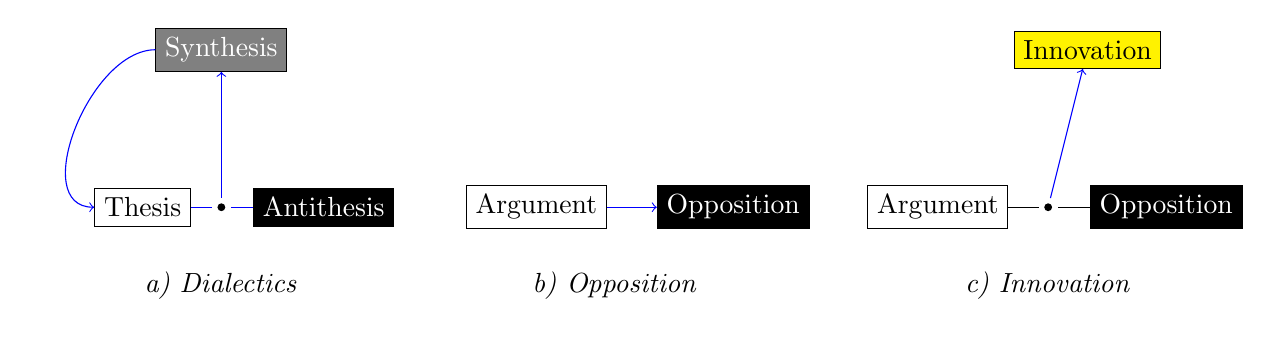
\begin{tikzpicture}
  % Dialectics
  \node[draw] (Thesis) at (0,0) {Thesis};
  \node[draw,fill=black,text=white] (Antithesis) at (2.3,0) {Antithesis};
  \node[draw,fill=gray,text=white] (Synthesis) at (1,2) {Synthesis};
  
  \draw node[vertex] (Joint) at (1,0) {};
  
  \draw[-,draw=blue] (Thesis) to (Joint);
  \draw[-,draw=blue] (Antithesis) to (Joint);
  \draw[->,draw=blue] (Joint) to (Synthesis);
  \draw[->,draw=blue] (Synthesis) to[in=180,out=180] (Thesis);
  
  \node at (1.0, -1.0) {\textit{a) Dialectics}};
  
  % Opposition
  \node[draw] (ArgumentA) at (5,0) {Argument};
  \node[draw,fill=black,text=white] (ArgumentB) at (7.5,0) {Opposition};
  
  \draw[->,draw=blue] (ArgumentA) to (ArgumentB);
  
  \node at (6., -1.0) {\textit{b) Opposition}};
  
  % Innovation
  \node[draw] (ArgumentA) at (10.1,0) {Argument};
  \node[draw,fill=black,text=white] (ArgumentB) at (13,0) {Opposition};
  \node[draw,fill=yellow] (ArgumentC) at (12,2) {Innovation};
  
  \draw node[vertex] (Joint) at (11.5,0) {};
  
  \draw[-] (ArgumentA) to (Joint);
  \draw[-] (ArgumentB) to (Joint);
  \draw[->,draw=blue] (Joint) to (ArgumentC);
  
  \node at (11.5, -1.0) {\textit{c) Innovation}};
\end{tikzpicture}
%\end{document}